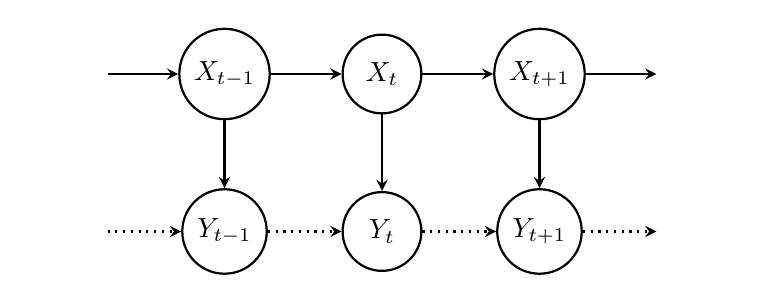
\begin{tikzpicture}[->, >=stealth, thick, node distance=2cm, every node/.style={circle, draw, minimum size=1cm}]

    % empty nodes 
    \node[draw=none] (Xtm2) at (-4,2) {};
    \node[draw=none] (Xtp2) at (4,2) {};
    \node[draw=none] (Ytm2) at (-4,0) {};
    \node[draw=none] (Ytp2) at (4,0) {};

    % Nodes for X_t
    \node (Xtm1) at (-2,2) {$X_{t-1}$};
    \node (Xt) at (0,2) {$X_t$};
    \node (Xtp1) at (2,2) {$X_{t+1}$};

    % Nodes for Y_t
    \node (Ytm1) at (-2,0) {$Y_{t-1}$};
    \node (Yt) at (0,0) {$Y_t$};
    \node (Ytp1) at (2,0) {$Y_{t+1}$};

    % Arrows for X_t dependencies
    \draw[thick] (Xtm2) -- (Xtm1);
    \draw[thick] (Xtm1) -- (Xt);
    \draw[thick] (Xt) -- (Xtp1);
    \draw[thick] (Xtp1) -- (Xtp2);

    % Arrows for Y_t dependencies
    \draw[thick] (Xtm1) -- (Ytm1);
    \draw[thick] (Xt) -- (Yt);
    \draw[thick] (Xtp1) -- (Ytp1);

    % Dotted arrow for Y_t-1 to Y_t
    \draw[dotted, thick] (Ytm2) -- (Ytm1);
    \draw[dotted, thick] (Ytm1) -- (Yt);
    \draw[dotted, thick] (Yt) -- (Ytp1);
    \draw[dotted, thick] (Ytp1) -- (Ytp2);

\end{tikzpicture}
